%Capítulo 1 - Introdução%

\thispagestyle{fancy}

\section{Contextualização}
O grande avanço tecnológico nas áreas de telecomunicação e eletrônica, apoiadas pelo desenvolvimento da física aplicada, fez com que os sinais transmitidos, em grande, parte migrassem para o meio digital. Hoje, a maior parte dos sistemas de comunicações já é digital \cite{john2001digital} .

Uma mensagem digital não é nada mais do que uma sequência ordenada de símbolos produzidos por uma fonte de informação discreta \cite{carlson2002introduction}. Entende-se por canal discreto o cascateamento Modulador-Canal-Demodulador, de modo que a entrada e a saída do canal são símbolos discretos. Um sistema de comunicação digital pode ser representado de acordo com a Figura 1.1.


\begin{figure}[!ht]
\begin{center}
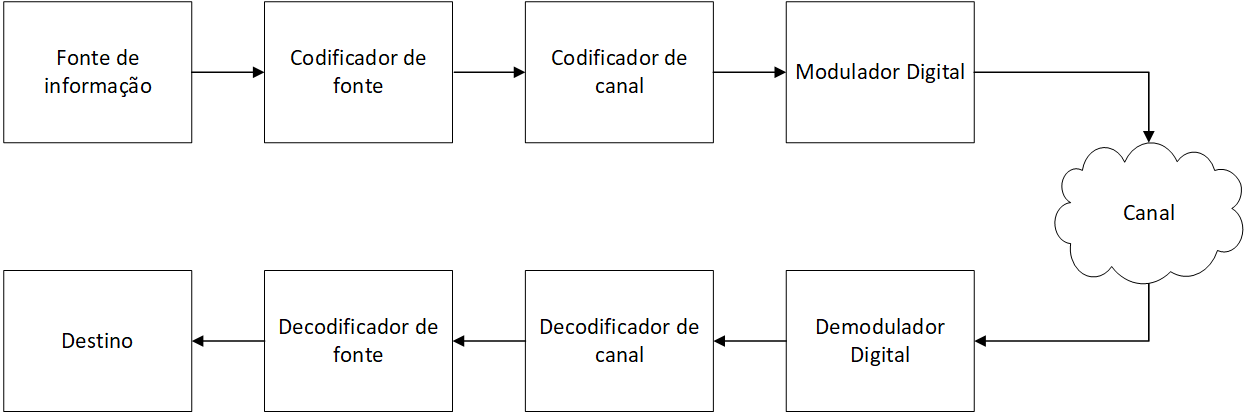
\includegraphics[scale=0.5]{./Figures/png/figura1.png}
\caption{Esquema em blocos de um sistema de comunicação digital.}
\label{fig:image_seq}
\end{center}
\end{figure}


Ao passar pelo canal, o sinal transmitido pode ser corrompido de forma aleatória por diversos mecanismos: adição de ruídos, atenuação, seletividade em frequência, deslocamento de fase, que são, em geral, dependentes do tempo. Estes diversos mecanismos podem comprometer a comunicação entre os dispositivos. 
 
Neste contexto, o uso de simulação é muito importante, pois a adoção de um padrão só é possível a partir do estudo, simulação e prototipação de um modelo definido. Para os sistemas de comunicação digitais, o desenvolvimento e teste de sistemas digitais, a comparação de desempenho de diferentes modelos de modulação, as restrições de custo nos testes e a necessidade de reproduzir condições ambientais onde o cenário possa ser repetido uma infinidade de vezes, dependem do suporte das simulações. 

\section{Justificativa e Motivações}

No desenvolvimento de modelos de comunicação, uma das técnicas mais empregadas consiste na simulação. Esta técnica, é considerada muito útil ao oferecer segurança na minimização de riscos e custos com diversos recursos e ações \cite{shannon1998introduction}.

A simulação é útil na resolução de problemas complexos que podem envolver situações determinísticas ou estocásticas. A simulação uma importante ferramenta de planejamento que procura emular, por meio de relações lógicas, o funcionamento de sistemas reais, a fim de observar seu comportamento sob diferentes cenários.

Os investimentos com modificações de produtos, processos, tecnologias e arranjos físicos são altos e arriscados. A simulação permite uma visualização mais detalhada do funcionamento da planta e ainda testes com cenários alternativos para indicar soluções a baixo custo, através de modelos computacionais.

Na área acadêmica a simulação possibilita estudar, em um ambiente virtual, o comportamento estático e dinâmico do modelo permitindo, dessa forma, projetar e prever a resposta do sistema sob investigação nas condições de trabalho que irão ocorrer no mundo real. A simulação, dessa forma, se apresenta, muitas vezes, como uma alternativa para reproduzir virtualmente experimentos que seriam muito onerosos.

Nesse contexto, a motivação deste TCC é: criar um software para simulação de um sistema de comunicação Digital utilizando faixa de frequência de 5 GHz. Para realizar este trabalho foi necessário a pesquisa de diversos pontos desta comunicação em artigos científicos e o aperfeiçoamento nas habilidades de programação em GNU Octave. 

\section{Objetivos}

Este trabalho propõe implementar um software que será utilizado para um ambiente de simulação de um sistema de comunicação digital usando o GNU Octave. O GNU Octave é uma Linguagem de Programação Científica que por ser um software livre que pode ser instalado gratuitamente em qualquer computador. Atualmente, está na versão 5.2.0. O GNU Octave pode ser executado em Windows, Linux e Mac OS \cite{octave}. 

Neste ambiente são abordados e comparados alguns parâmetros utilizados em um sistema de comunicação digital, tais como técnicas de modulação, nível de ruído na transmissão, entre outros. 

\section{Trabalhos Relacionados }

No trabalho de Aquino (2012) \cite{aquino2012modelo}, descreve a implementação de um sistema de comunicação digital usando o software Scilab, e levanta a possibilidade do software desenvolvido poder ser usado como ferramenta auxiliar em diversas disciplinas dos cursos técnicos em telecomunicações, tecnólogo em telemática, engenharia de telecomunicações. 

No estudo de Neto (2016) \cite{netoaprendendo}, cujo título é “APRENDENDO NA PRÁTICA: USO 
DO MATLAB® NO ESTUDO DA TAXA DE ERRO DE SÍMBOLO EM MODULAÇÕES M-ÁRIAS COM DETECÇÃO COERENTE”, nos apresenta a necessidade de meios de simulação em cursos de engenharia e demonstra a capacidade da integração lógica e prática por meio do auxílio da ferramenta Matlab® como escape para a ausência da prática. 

O trabalho de Cantu (2018) \cite{Cantur:2018:IFSC} propõe a implementação de um toolbox de funções de sincronismo de símbolo para a plataforma GNU Octave, este trabalho usuário possa migrar suas simulações que utilizam sincronizações da plataforma proprietária para a plataforma gratuita. 

Dentre várias pesquisas e protótipos desenvolvidos neste escopo, várias plataformas de simulação utilizadas e validadas como Scilab Aquino (2012) \cite{aquino2012modelo} e Matlab Yuting (2016) \cite{yuting2010simulation}, entretanto há uma carência de trabalhos utilizando GNU Octave. 

Neste trabalho, detectou-se a necessidade de ampliação dos estudos, através da implementação de um sistema de comunicação digital utilizando outra plataforma para simulação gratuita e de código livre, neste trabalho foi escolhido o GNU Octave. 
